\chapter{Syntax}\label{chap:syntax}

To describe the formal syntax of \gls{gamble}, and to parse the language, it is necessary to write a \acrfull{cfg}.
This chapter will explain what a \acrshort{cfg} is, and the problems encountered while creating one.
After this an explanation of \gls{gamble}'s \acrshort{cfg}, will be presented.

\section{Context-Free Grammar}\label{sec:cfg}
\acrshort{cfg} is formal grammar used to specify the syntax of a language.
A \acrshort{cfg} consists of one or more production rules.
On the left side of a production rule is a non-terminal and on the right side are terminals and/or non-terminals, one of the non-terminals is also known as the start symbol of the \acrshort{cfg}.
An example of this is written in \myref{lst:cfglst1}, where a definition for multiplication and addition including parenthesis is shown.
The expression production on this figure uses left recursion, since an expression has a production which first element is also an expression.
The grammar is structured such that the multiplication operator have a higher precedence than the addition operator, because \texttt{term} is located before the production rule using the \texttt{+} symbol.

\begin{lstlisting}[caption={An example of a \acrshort{cfg} written in \acrshort{ebnf}, with \acrshort{regex} for defining numbers. },frame=tlrb,label={lst:cfglst1},numbers=none]
expression : term 
           | expression "+" term;
term       : factor 
           | term "*" factor;
factor     : constant 
           | "(" expression ")";
constant   : [0-9]+
\end{lstlisting}

It is possible to generate a parse tree for a string which follows the grammar.
A parse tree is a tree which shows the derivation for a string from the start symbol of the \acrshort{cfg} until all the leafs of the tree only contains terminal of the \acrshort{cfg}. 
In translators this is done using what is called a parser, which is a program that transforms strings into parse trees. 
This will further be explained in \myref{sec:parsetrees}.
If there exists two or more parse trees for any given string then the grammar is ambiguous. 
Having an ambiguous grammar can be a problem when parsing because one cannot always decide which grammar rule it should apply.

\subsection{The dangling else problem} 
This section shows an example of how to solve the problem of ambiguity for grammars. 
Some tools for generating parsers from grammars, can solve these problems themselves.

A common mistake leading to ambiguous grammar is the dangling else problem. \citep{danglingelse}
In many programming languages it is possible to have an if statement and an else statement, and inside the body of these also having if- and else statements. 
A \acrshort{cfg} describing it is shown in \myref{lst:danglingelseex1}.

\begin{lstlisting}[caption={An example of a \acrshort{cfg} describing an if statement. \citep{danglingelse}},frame=tlrb,label={lst:danglingelseex1},numbers=none]
if statement :
    | if clause statement
    | if clause statement else statement

statement :
    | simple statement
    | if statement
    | loop statement
\end{lstlisting}

Given an input where the statement of an if statement contains another if statement this grammar is ambiguous.  
However it can be rewritten to allow if-else statements in a grammar, yet this will in almost all cases cause the size of the grammar to increase. 
A solution to this problem is to observe that there exists two kinds of if statements, open and closed if statements.
An open statement is one in which the if statement is not paired with an else, and a closed statement is any if statement paired with an else.
A simple statement is also a closed statement and it is also any regular statement, i.e. assignment.
\myref{lst:danglingelseex2} shows a grammar resolving the dangling else problem using this method.


\begin{lstlisting}[caption={An example of a \acrshort{cfg} describing an if statement, that is not ambiguous. \citep{danglingelse}},frame=tlrb,label={lst:danglingelseex2},numbers=none]
statement :
    | open statement
    | closed statement

open statement :
    | if clause statement
    | if clause closed statement else open statement

closed statement :
    | simple statement
    | if clause closed statement else closed statement
\end{lstlisting}

Another way to resolve this issue is to force statement bodies of if statements, when followed by an else statement, to be delimited by explicit blocks, such as \texttt{begin..end} used in Pascal or curly brackets (\texttt{\{\ldots\}}) used in C and derivatives. 

\subsection{Derivations of parse trees}\label{sec:parsetrees}
A parser is a program which takes a string of symbols, and parses it into segments according to the rules specified in a grammar.
A more thorough explanation of parsers and specifically the one implemented for this project can be found in \myref{subsec:parser}.
Two common strategies to generate a parse tree is leftmost derivation and rightmost derivation. 
A leftmost derivation applies the rules in the grammar by always applying a production rule to the leftmost non-terminal. 
This is the strategy used in a top-down parser, also known as an LL parser.
A rightmost derivation is the reverse, and what is used in a bottom-up parser, also known as a LR parser.
An LL is a subset of LR, and as such an LR parser can also parse LL languages. 

\section{Classes of CFGs}
As mentioned there are two common strategies for parsing, leftmost and rightmost. 
A parser has a lookahead which is the maximum numbers of tokens, which are groups of symbols, and are needed to determine what rule should be applied, this is denoted in a parenthesis, so e.g. LL(1) means leftmost derivation using a lookahead of 1 token.
A lookahead of \emph{k} means that there is a constant lookahead of a maximum of \emph{k} tokens for the given parser. 
LL(*) is also a grammar class, which can dynamically change the number of tokens needed to parse by recognising if they follow a \acrlong{regex}.
An LL parser is called an LL(*) parser if it is not limited to finite \emph{k} tokens of lookahead, but can make parsing decisions by recognising whether the following tokens belong to a regular language.
Combining this with the fact that any LL grammar is a subset of an LR grammar and the different cases of lookahead constructs a diagram. 
This Venn diagram is shown in \myref{fig:hierarchyofgrammars}, LL(*) can express the same grammars as LL(k).

\begin{figure}[!ht]
\centering
 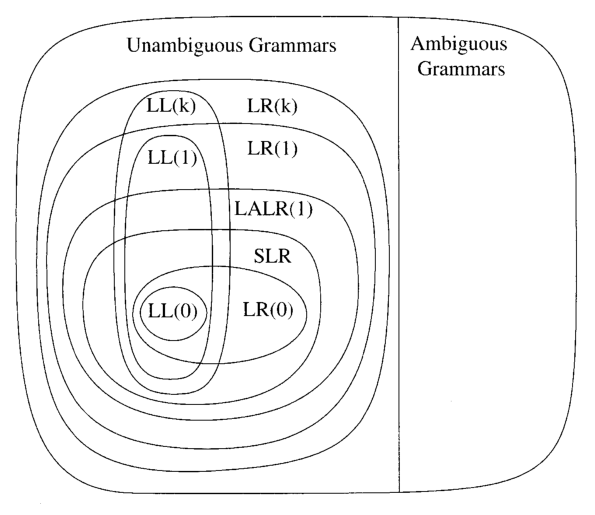
\includegraphics[width=0.5\textwidth]{figures/classesofgrammars.png} % trim=4.85cm 15cm 0.85cm 1cm
\caption[A Venn diagram showing the similarities between the different subclasses of CFGs]{A Venn diagram showing the similarities between the different subclasses of CFGs. Where LL(*) is marked with light blue. \citep{Lecture5}}
\label{fig:hierarchyofgrammars}
\vspace{-15pt}
\end{figure}
\section{Context free grammar in GAMBLE}
\gls{gamble}'s grammar is written in \acrfull{ebnf}, and uses regular expressions to define terminals such as numbers and identifiers.
In this section there will be a short traversal of a branch from the parse tree.\todo{Hvad ? hvad betyder det??? - Søren}
The full \acrshort{cfg} of \gls{gamble} can be found in \myref{app:CFG} alongside the lexing rules.
This section only presents a small selection of the \acrshort{cfg}.
\gls{gamble}s \acrshort{cfg} is used in the compiler for parsing a program into a structure, which can be manipulated and analysed to produce the target code for the specific program.\todo{Er det vigtigt ? Kan vi ikke nøjes med at sige at grammatikken skal bruges til en parser for gamble ? Vi forklarede det jo i sidste afsnit ? - Søren}
The production rules are used to check for any syntactical errors which might occur.

A production rule from the \acrshort{cfg} of \gls{gamble} is the statement rule. 
Looking at \myref{lst:statements} it is seen that a statement can be both an assignment, declaration, functioncall, controlblock or a loop construct. 
Statement productions are the building blocks of any source code written in \gls{gamble}.

\begin{lstlisting}[caption={\acrshort{cfg} Statement},frame=tlrb,label={lst:statements},numbers=none]
statement
    : assignment ';'
    | declaration ';'
    | functioncall ';'
    | controlblock 
    | loop
    ;
\end{lstlisting}

All production rules in the statement each expand to their own production hence they are non-terminals.
Looking at the declaration production on \myref{lst:declaration} observe that it has two production rules, \texttt{datatype '=' expression} and \texttt{complexdatatype ID '=' expression}. 
They both end on the expression production which can be seen on \myref{lst:expression}.

\begin{lstlisting}[caption={\acrshort{cfg} Declaration},frame=tlrb,label={lst:declaration},numbers=none]
declaration
    : datatype ID '=' expression                        #primitiveDecl
    | complexdatatype ID '=' expression                 #complexDecl
    ; ;
\end{lstlisting}\todo{Er denne rigtig i forhold til den nye grammatik der er blevet lavet igennem tiden ? Den opdaterede grammatik skal også sættes ind i appendix - Søren}

Further expanding into the expression production rules, it can be seen that it has five different production rules.
An expression has production rules expanding the expression into a construct containing more expressions.
This is done because an expression can derive to a value, and several values are needed for multiple arithmetic operations.
This construct also causes left-recursion, something often attempted to be avoided in \acrshort{cfg}.
The parse generator \acrshort{antlr} can handle simple left-recursion as seen on \myref{lst:value} and as such it is acceptable in the \acrshort{cfg} for \gls{gamble}.\todo{Måske vi skal have et afsnit inden gamble CFG omkring parse generators eller noget ? :) Det skal bare nævnes et sted - Søren}
It does so internally rewriting it and as such removes the left-recursion.
\begin{lstlisting}[caption={\acrshort{cfg} Expression},frame=tlrb,label={lst:expression},numbers=none]
expression
    : expression ( '*' | '/' | '%' ) expression     #mulExpr
    | expression ( '+' | '-' ) expression           #addExpr
    | '(' expression ')'                            #parenExpr
    | value                                         #valueExpr
    | ID postUnaryOperator                          #postIDExpr
    ;
\end{lstlisting}
  
The value production rule can expand into what is seen on \myref{lst:value}.
In this production both terminals and non-terminals are included.
The terminals are elements that have no further production rules, leading to a ``dead end''.
When a terminal is reached it is encountered the deriviation ends and the terminal becomes a leaf on the parse tree, also seen in \myref{sec:AST}.
\begin{lstlisting}[caption={\acrshort{cfg} Value},frame=tlrb,label={lst:value},numbers=none]
value
    : ID                                     #valID
    | constant                               #valConstant
    | '[' valueList ( ';' valueList )* ']'   #valList
    | functioncall                           #valFuncCall
    | collectionEntrance                     #valCollectionEntrance
    | BOOLVAL                                #valBool
    ;
\end{lstlisting}\todo{Er de rent faktisk terminals ? Er en terminal ikke noget som ikke har en productionrule ? Det har de vel allesammen her ?}
\todo[inline]{burde vi ikke beskrive alternative labels aka hashtags #? MP}


